\subsection{Running-Time Analysis}

\subsubsection{Theoretical Analysis}

Let $T(n)$ be the running time of
\textsc{Max-Subarray} on $n$ minutes of data.

For $n = 1$ the algorithm performs a constant
amount of work, so $T(1) = \Theta(1)$.

For $n \ge 2$, computing $mid$ takes $O(1)$ time,
the two recursive calls are on ranges of length
$\lceil n/2 \rceil$ and $\lfloor n/2 \rfloor$, and
\textsc{Max-Crossing} visits each of the $n$
elements of the range exactly once, taking
$\Theta(n)$ time. Choosing the best of three
candidates takes $O(1)$ time. Therefore

\[
T(n) = T(\lceil n/2 \rceil) + T(\lfloor n/2 \rfloor)
+ \Theta(n).
\]

This recurrence has the form
$T(n) = aT(n/b) + f(n)$ with $a = 2$, $b = 2$, and
$f(n) = \Theta(n) = \Theta(n^{\log_b a})$.
By case~2 of the Master Theorem
\cite[Sec.~4.5]{clrs2009} (floors and ceilings do
not affect the asymptotic solution
\cite[Sec.~4.6]{clrs2009}),

\[
\boxed{T(n) = \Theta(n \log n)}
\]

The same bound follows from the recursion tree.
The subproblems at any fixed depth are disjoint
ranges of $[1, n]$, so the crossing scans at that
depth visit at most $n$ elements in total, and the
tree has depth $\lceil \log_2 n \rceil$.
When $n$ is a power of two, every level above the
leaves visits exactly $n$ elements, so the crossing
loops perform exactly $n \log_2 n$ additions.
This count does not depend on the values $x_i$, so
the bound holds for every input, not only in the
worst case.

The recursion makes $2n - 1$ calls in total, each
doing $O(1)$ work outside the crossing loops,
contributing an additional $\Theta(n)$ term.
The extra space is $O(\log n)$ for the recursion
stack, since the algorithm works on index ranges
of the original array and never copies it.

\subsubsection{Experimental Verification}

The algorithm was implemented in C++ and tested
on randomly generated per-minute net queue changes,
drawn uniformly from $-30$ to $+30$ vehicles.

Eleven input sizes were tested, ranging from
10,000 to 16,000,000 minutes.
For each input size the measurement was repeated
10 times and the median was recorded.
Because the smallest inputs complete faster than
the resolution of the system clock, each measurement
runs the algorithm $\max(1, \lfloor 4\cdot 10^6 / n \rfloor)$
times and reports the average time per run.

Timing used the C++ \texttt{chrono} steady clock,
input generation was excluded from the timed
region, and the program was compiled with
\texttt{g++ -O2}.

Before timing, the implementation was checked
against an $O(n^2)$ brute-force search on 2,000
random inputs of length 1 to 60, and every
benchmark answer was checked against an
independent $O(n)$ scan \cite{bentley1984}.
All checks passed.

\begin{table}[htbp]
\centering
\caption{Divide-and-Conquer Running-Time Results}
\label{tab:dc-runtime}
\begin{tabular}{|r|r|r|}
\hline
Input Size ($n$) & Median Time (ms) & Time$/n$ (ns) \\
\hline
10,000 & 0.247 & 24.7 \\
20,000 & 0.553 & 27.6 \\
50,000 & 1.464 & 29.3 \\
100,000 & 2.964 & 29.6 \\
200,000 & 6.135 & 30.7 \\
500,000 & 15.607 & 31.2 \\
1,000,000 & 31.756 & 31.8 \\
2,000,000 & 64.925 & 32.5 \\
4,000,000 & 130.957 & 32.7 \\
8,000,000 & 272.306 & 34.0 \\
16,000,000 & 528.324 & 33.0 \\
\hline
\end{tabular}
\end{table}

\subsubsection{Experimental Graph}

Figure~\ref{fig:dc-runtime} (top) compares the
measured execution times with an $n\log n$ curve
scaled to match the largest input, and with the
fitted model $T(n) = a\,n\log_2 n + b\,n$.

Because $n\log n$ and $n$ differ only by a slowly
growing factor, the bottom plot shows the
normalized time $T(n)/n$ against $\log_2 n$.
If $T(n) = a\,n\log_2 n + b\,n$, this plot is a
straight line with slope $a$; a purely linear
algorithm would instead give a horizontal line.

\begin{figure}[htbp]
\centering
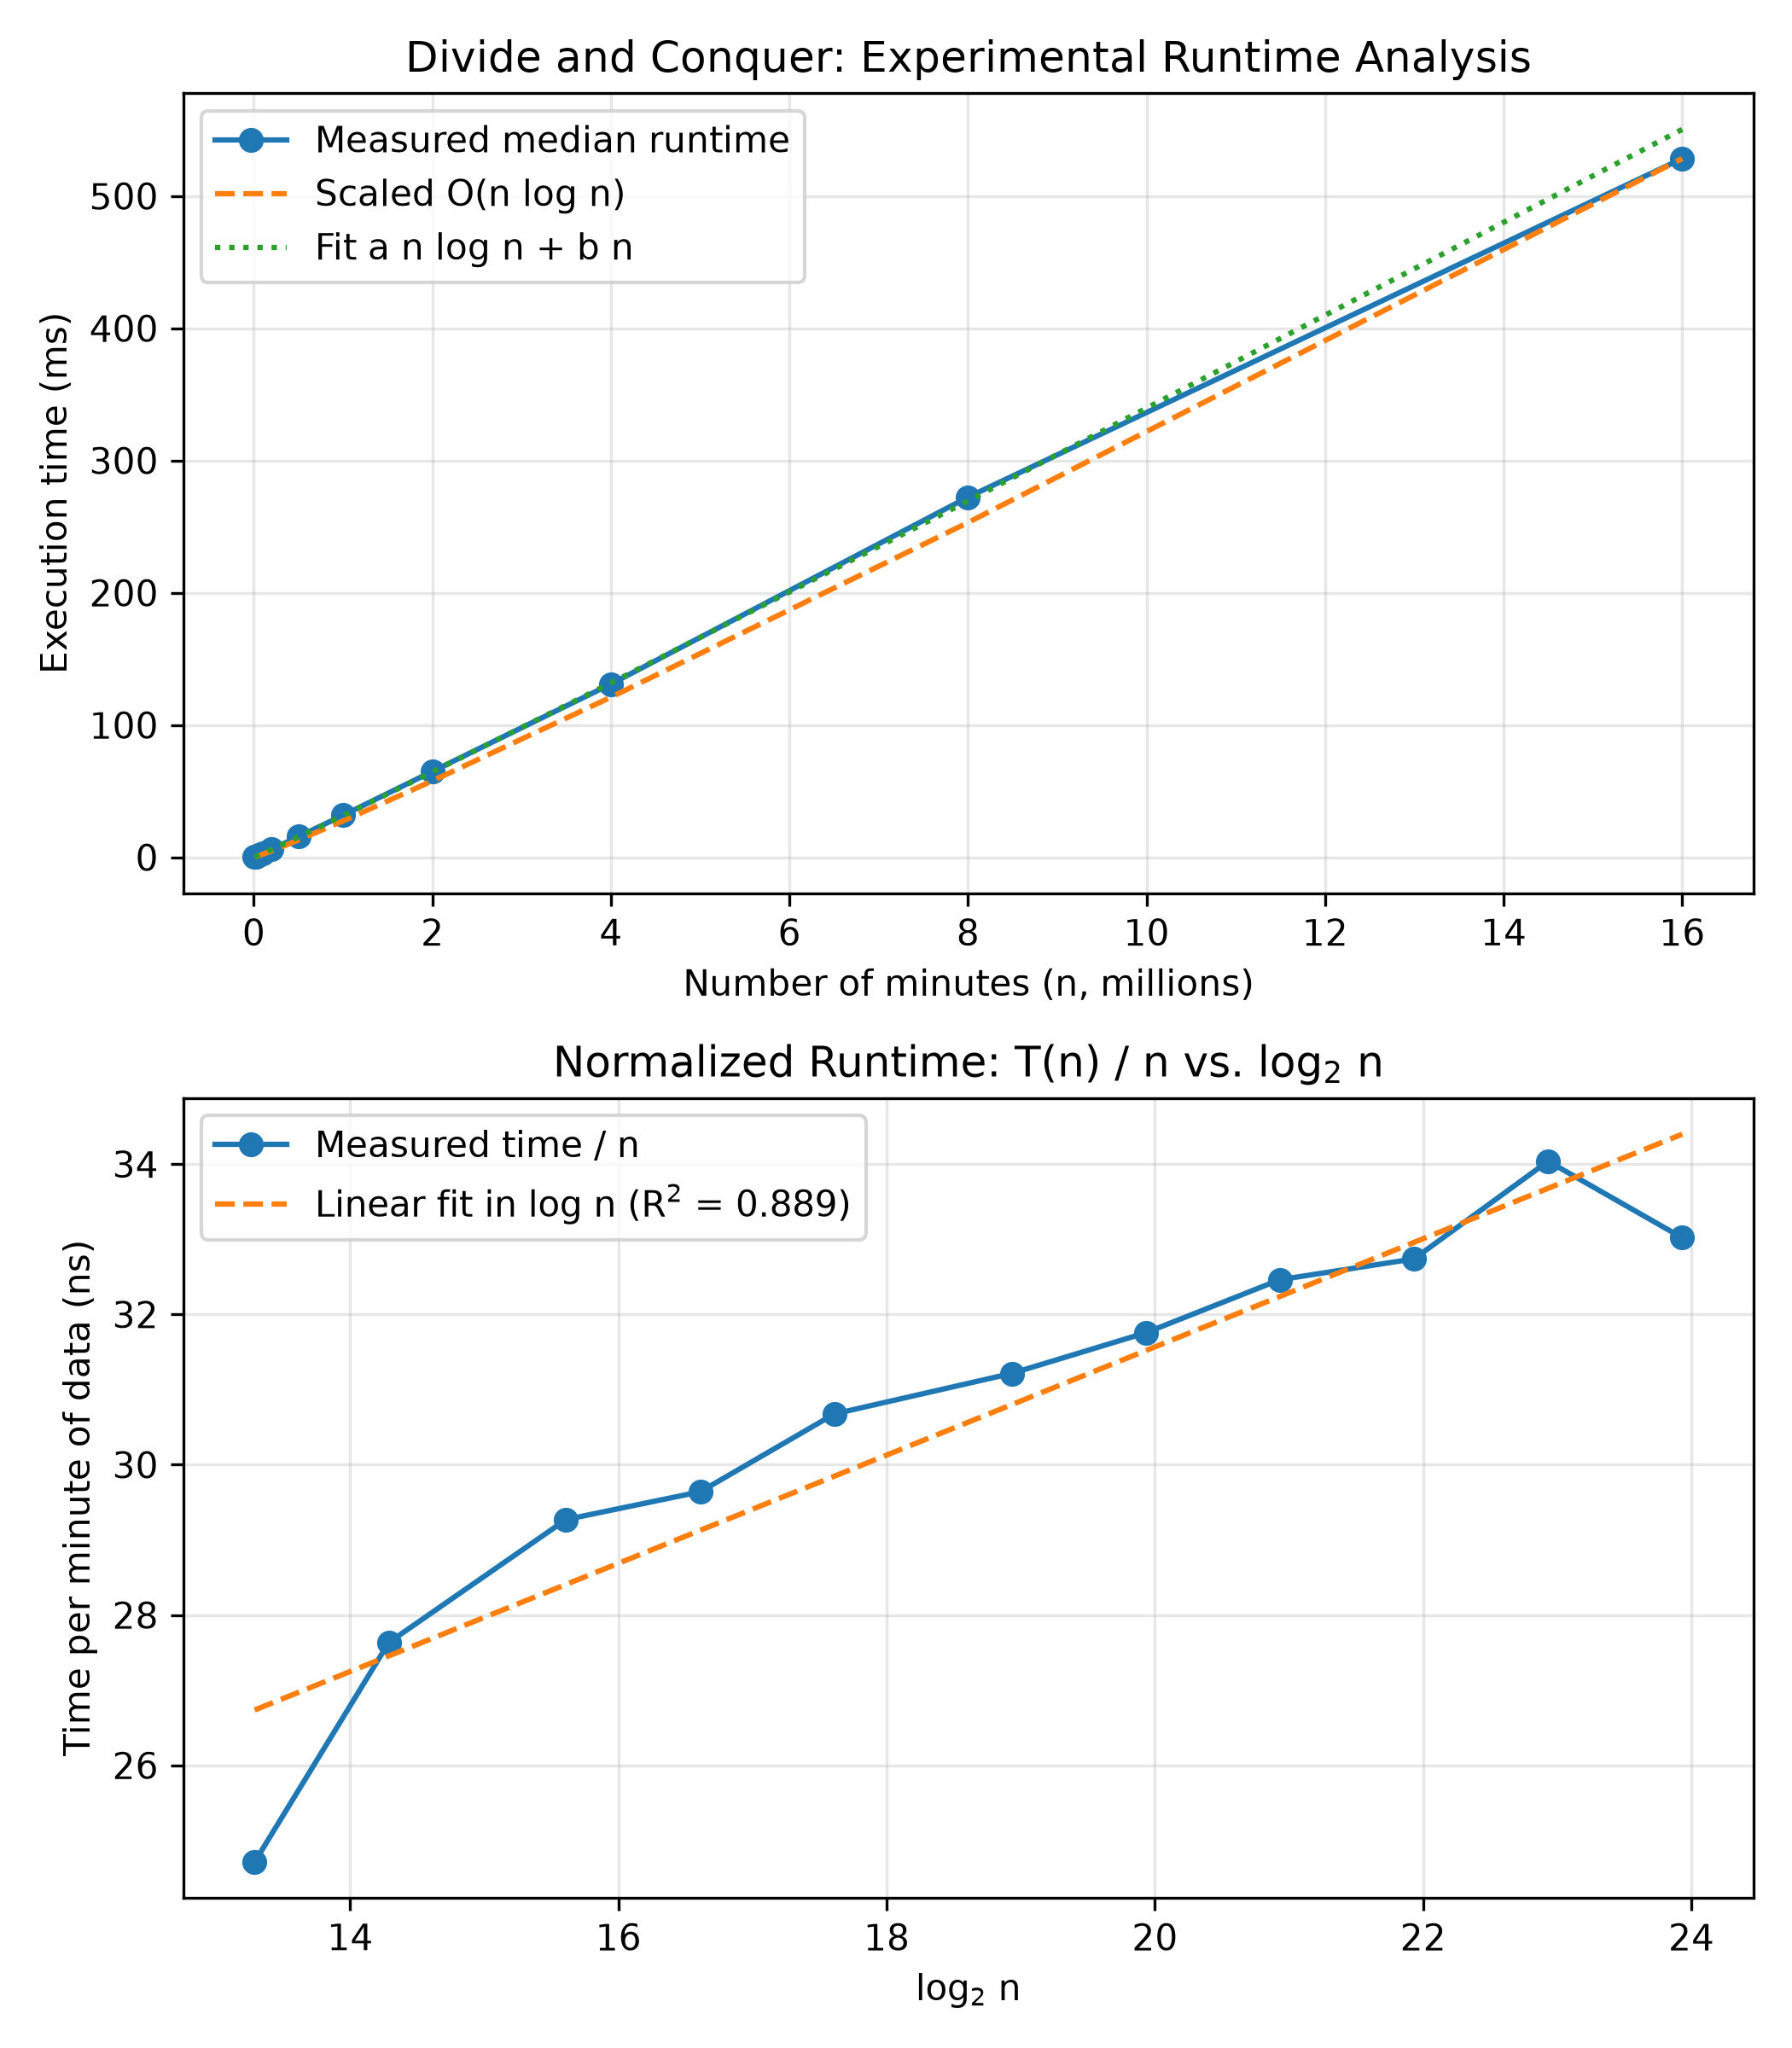
\includegraphics[width=\linewidth]{dc_runtime_graph.png}
\caption{Top: measured median execution time of
the divide-and-conquer algorithm compared with
scaled $n\log n$ growth. Bottom: time per minute
of data versus $\log_2 n$.}
\label{fig:dc-runtime}
\end{figure}

The normalized time increases steadily with
$\log_2 n$. A least-squares fit gives
$T(n)/n \approx 0.72\log_2 n + 17.2$ ns with
$R^2 = 0.889$, i.e., a positive $n\log n$
coefficient, consistent with the
$\Theta(n\log n)$ analysis.

The intercept shows that the $\Theta(n)$ term from
the $2n - 1$ recursive calls has a large constant
compared with the inexpensive additions in the
crossing loops, which is why the absolute times
in the top plot look close to linear over this
range.

Deviations from the fitted line, such as the lower
time per element at $n = 10{,}000$ (where the whole
input fits in the processor cache) and the
fluctuation at the two largest sizes, are attributed
to memory-hierarchy effects and system activity.
